

    %https://tex.stackexchange.com/questions/167719/how-to-use-background-image-in-latex


    \documentclass{article}

    %Tipo de letra parecido a tahoma
    %sudo apt install texlive-fonts-extra
    \usepackage[default]{roboto} 

    %package needed for the background
    \usepackage{eso-pic,graphicx}

    %defining the margins and the page size
    \usepackage[top=0cm, bottom=0cm, outer=0cm, inner=0cm, 
                letterpaper]{geometry}

    %package for formating numbers
    \usepackage{siunitx}

    %defining colors
    \definecolor{BlueDark}{RGB}{12,58,229}
    \definecolor{BlueDarkDark}{RGB}{5,71,127}
    \definecolor{BlueLight}{RGB}{0,195,255}
    \definecolor{GrayLight}{RGB}{179,179,179}
    \definecolor{GrayDark}{RGB}{102,99,91}

    %Command to insert text in the desired positions
    %https://tex.stackexchange.com/questions/168141/can-latex-place-text-by-mm-coordinates
    \usepackage{tikz}
    \newcommand\PlaceText[3]{%
    \begin{tikzpicture}[remember picture,overlay]
        \node[outer sep=0pt,inner sep=0pt,anchor=south west] 
            at ([xshift=#1,yshift=-#2]current page.north west) { #3};
    \end{tikzpicture}%
    }

    %Command to insert image in the desired positions

    \newcommand\PlaceFigure[3]{%
    \begin{tikzpicture}[overlay, remember picture]
    \node[anchor=north west, %anchor is upper left corner of the graphic
        xshift=#1, %shifting around
        yshift=-#2] 
        at (current page.north west) %left upper corner of the page
        {\includegraphics[]{#3}}; 
    \end{tikzpicture}%
    }
    
    \begin{document}
    
    %insert Background page 1
    %https://tex.stackexchange.com/questions/167719/how-to-use-background-image-in-latex
    \AddToShipoutPictureBG*{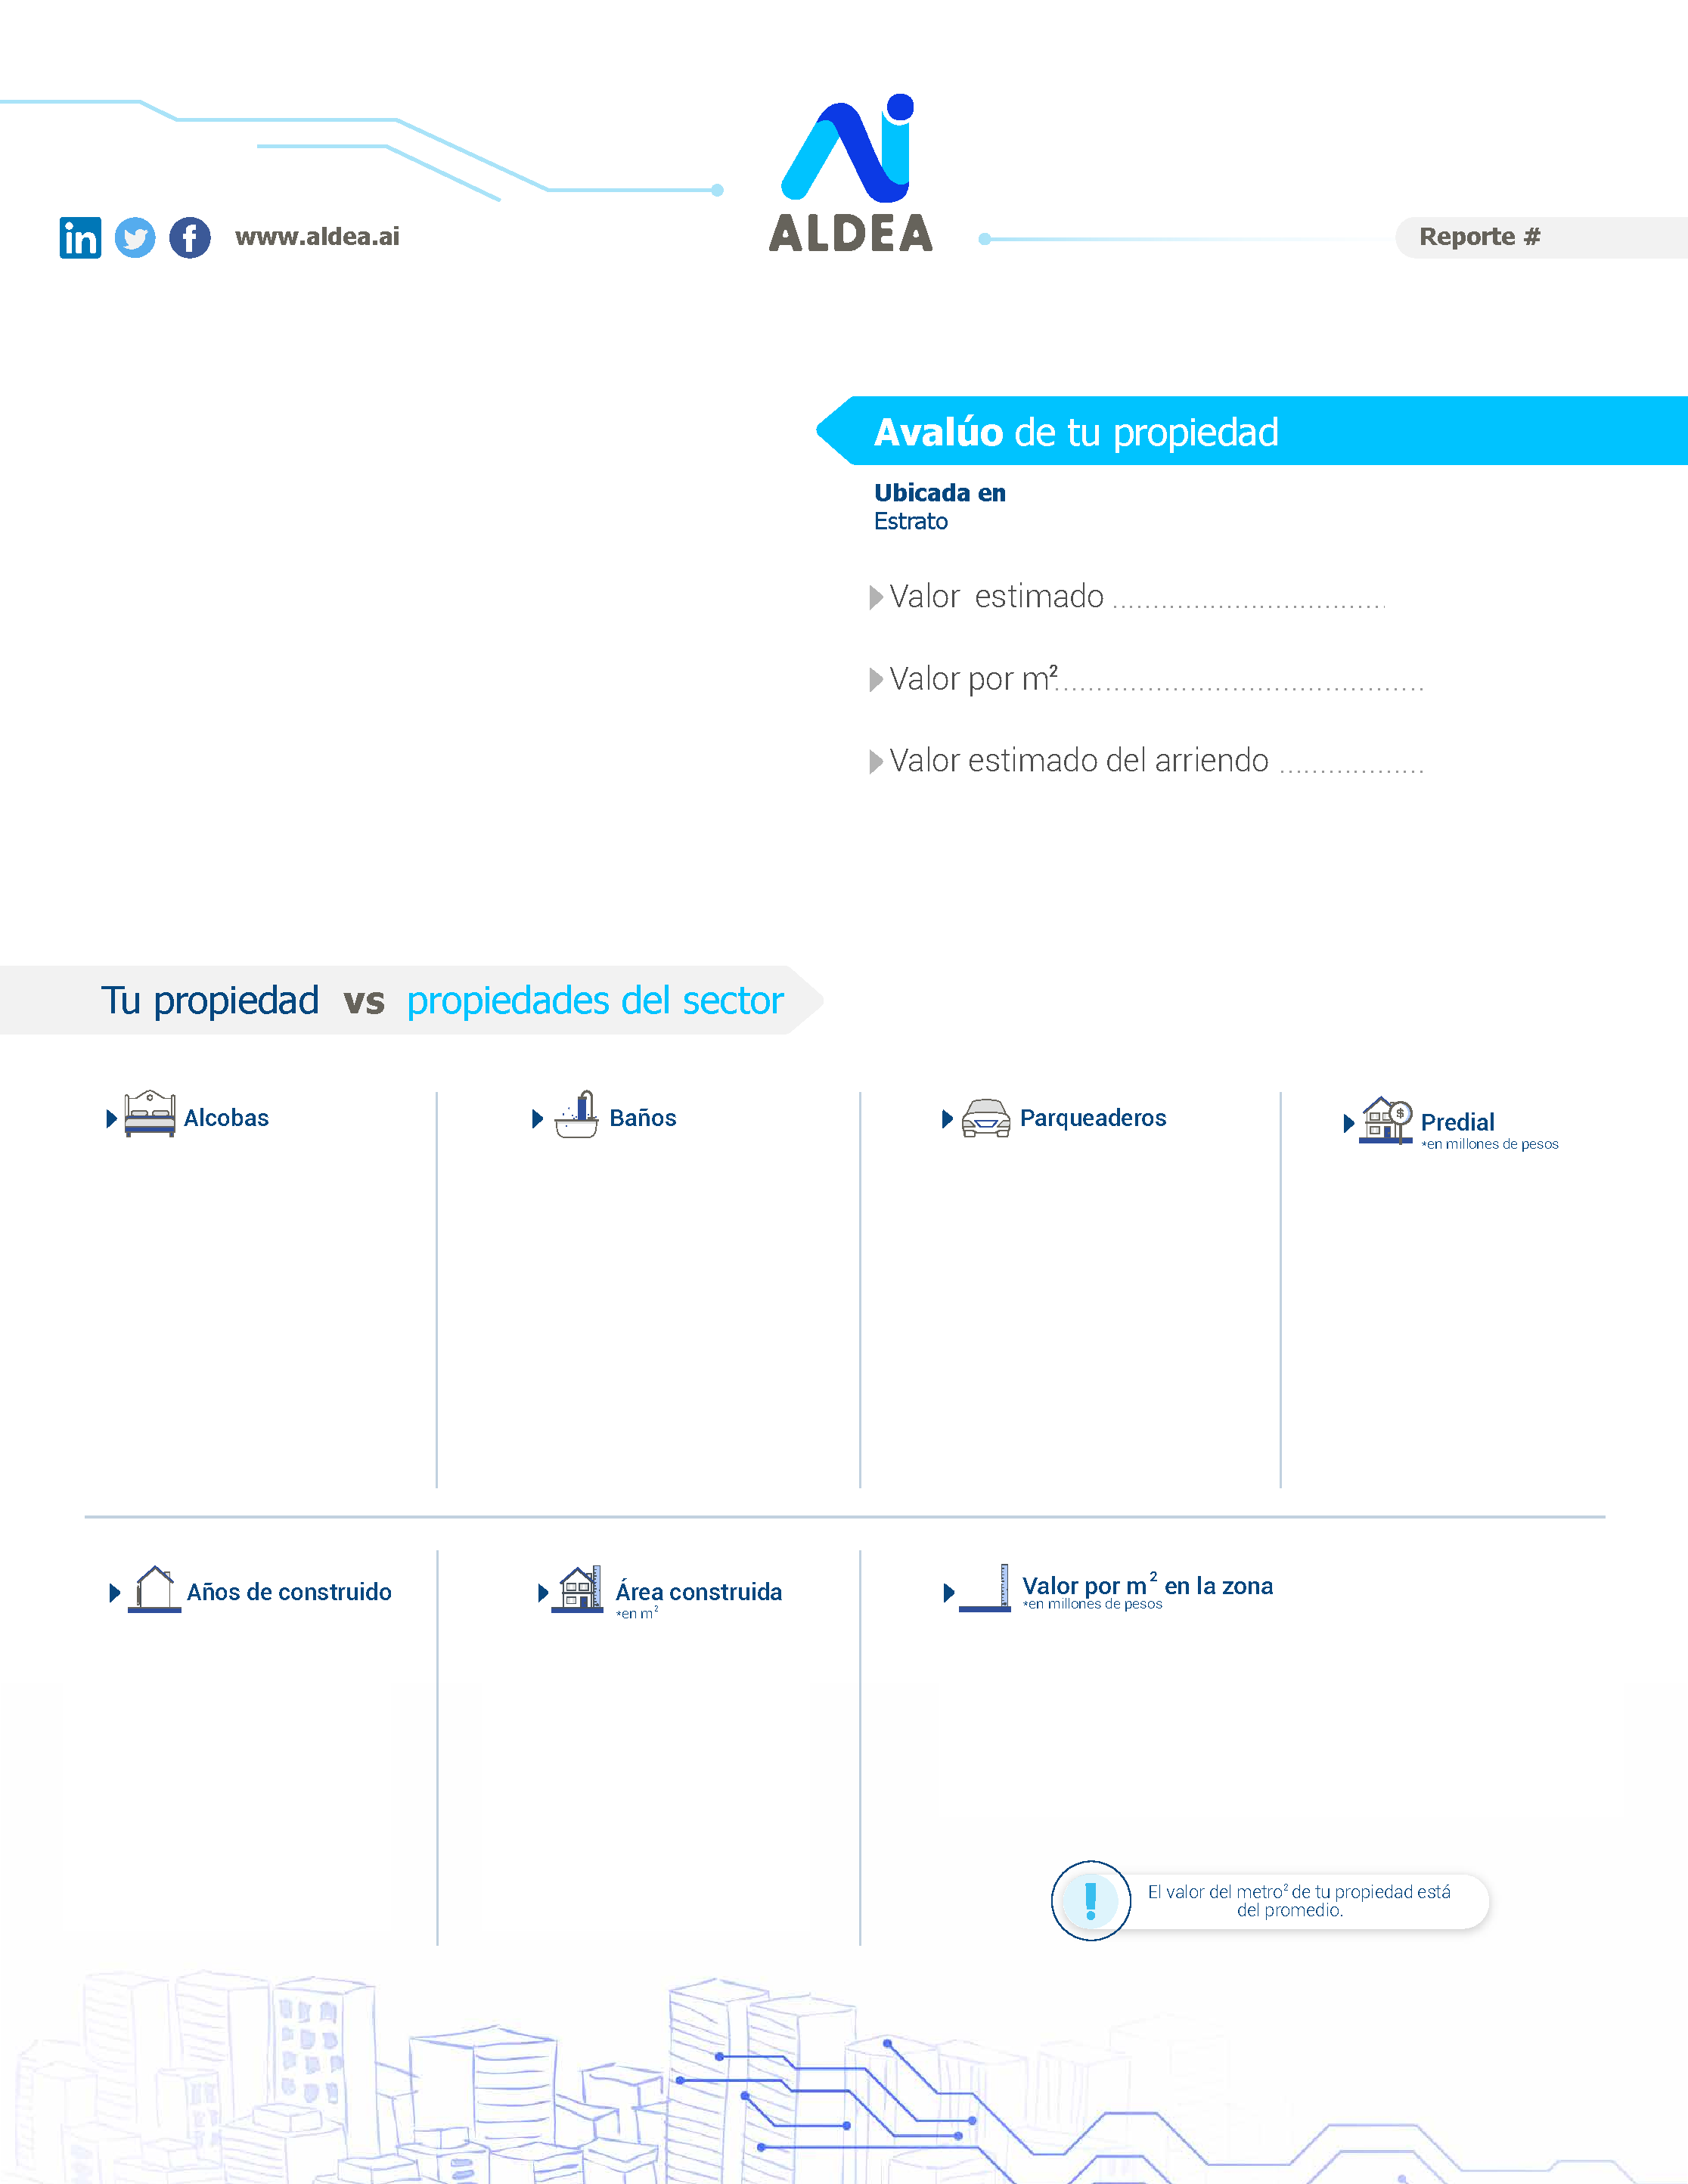
\includegraphics[width=\paperwidth, height=\paperheight, page=1]{ALDEAAIAVALUOV3plantillaSebas.pdf}}
    
    %%%%%%%%%%%%%%%%%%%%%%%%%%5
    %Inserting text

    %Numero de reporte
    \PlaceText{0.92\paperwidth}{0.113\paperheight}{{\textbf{\color{GrayDark} {1}}}}
    %Dirección
    \PlaceText{0.6\paperwidth}{0.2315\paperheight}{\color{BlueDarkDark} {Carrera 78 \# 34A - 56 Medellín, Colombia.}}
    %Estrato
    \PlaceText{0.567\paperwidth}{0.243\paperheight}{\color{BlueDarkDark} {5}}
    %Valor Estimado
    \PlaceText{0.7\paperwidth}{0.28\paperheight}{\large{{\color{BlueLight} {\$ \SI[]{326000000}{} - \$ \SI[]{360000000}{}}}}}
    %Valor por m2
    \PlaceText{0.7\paperwidth}{0.3175\paperheight}{\large{{\color{BlueLight} {\$ \SI[]{4600000}{} - \$ \SI[]{5100000}{}}}}}
    %Valor Estimado Arriendo
    \PlaceText{0.76\paperwidth}{0.355\paperheight}{\large{{\color{BlueLight} {\$ \SI[]{2100000}{} - \$ \SI[]{2300000}{}}}}}
    %Valor por m2 en la zona
    \PlaceText{0.677\paperwidth}{0.8795\paperheight}{\scriptsize{\textbf{\color{BlueDarkDark} {por debajo}}}}


    %%%%%%%%%%%%%%%%%%%%%%%%%%5
    %Inserting mages

    %Mapa
    \begin{tikzpicture}[overlay, remember picture]
    \node[anchor=north west, %anchor is upper left corner of the graphic
        xshift=0.0\paperwidth, %shifting around
        yshift=-0.174\paperheight] 
        at (current page.north west) %left upper corner of the page
        {\includegraphics[scale=0.5, trim=0 40 0 0, clip]{Mapa.png}}; 
    \end{tikzpicture}%


    %Alcobas
    \PlaceFigure{-0.047\paperwidth}{0.484\paperheight}{InfoAlcobas.png}

    %Banos 
    \PlaceFigure{0.206\paperwidth}{0.484\paperheight}{InfoBanos.png}

    %Parqueaderos
    \PlaceFigure{0.449\paperwidth}{0.484\paperheight}{InfoParqueaderos.png}

    %Predial
    \PlaceFigure{0.6866\paperwidth}{0.484\paperheight}{InfoPredial.png}

    %Anos de contruido
    \PlaceFigure{-0.047\paperwidth}{0.701\paperheight}{InfoAnoConstruccion.png}

    %Area Construida
    \PlaceFigure{0.206\paperwidth}{0.701\paperheight}{InfoAreaConstruida.png}

    %Valor por m2
    \PlaceFigure{0.525\paperwidth}{0.745\paperheight}{PricePerM2.png}

    \newpage
    

    %%%%%%%%%%%%%%%%%%%%%%%%%%5
    %%%%%%%%%%%%%%%%%%%%%%%%%%5

    %insert Background page 2
    %https://tex.stackexchange.com/questions/167719/how-to-use-background-image-in-latex
    \AddToShipoutPictureBG*{\includegraphics[width=\paperwidth, height=\paperheight, page=2]{ALDEAAIAVALUOV3plantillaSebas.pdf}}

    %%%%%%%%%%%%%%%%%%%%%%%%%%5
    %Inserting text
    
    %Alcobas
    \PlaceText{0.1025\paperwidth}{0.1659\paperheight}{\scriptsize{\textbf{\color{BlueDarkDark} {20\%}}}}\PlaceText{0.175\paperwidth}{0.1754\paperheight}{\scriptsize{\color{BlueDarkDark} {2}}}
    %Area construida
    \PlaceText{0.515\paperwidth}{0.1754\paperheight}{\scriptsize{\color{BlueDarkDark} {117m$^{2}$}}}
    %Valor Promedio
    \PlaceText{0.819\paperwidth}{0.1759\paperheight}{\scriptsize{\color{BlueDarkDark} {\$\SI[]{4900000}{}}}}
    %Valorización
    \PlaceText{0.515\paperwidth}{0.5877\paperheight}{\large{\textbf{\color{BlueDarkDark} {desvalorizado}}}}\PlaceText{0.355\paperwidth}{0.604\paperheight}{\large{\textbf{\color{BlueDarkDark} {7\%}}}}
    %Anexos
    \PlaceText{0.07\paperwidth}{0.744\paperheight}{\color{GrayDark} {No. de alcobas}}\PlaceText{0.24\paperwidth}{0.744\paperheight}{\color{GrayLight} {2}}\PlaceText{0.07\paperwidth}{0.765\paperheight}{\color{GrayDark} {No. de ba\~{n}os}}\PlaceText{0.24\paperwidth}{0.765\paperheight}{\color{GrayLight} {2}}\PlaceText{0.07\paperwidth}{0.786\paperheight}{\color{GrayDark} {No. de niveles}}\PlaceText{0.24\paperwidth}{0.786\paperheight}{\color{GrayLight} {1}}\PlaceText{0.07\paperwidth}{0.807\paperheight}{\color{GrayDark} {Valor administraci\'{o}n}}\PlaceText{0.24\paperwidth}{0.807\paperheight}{\color{GrayLight} {\$ \SI{299000}{} }}\PlaceText{0.38\paperwidth}{0.744\paperheight}{\color{GrayDark} {\'{A}rea terraza}}\PlaceText{0.55\paperwidth}{0.744\paperheight}{\color{GrayLight} {\SI{0}{\square\meter}}}\PlaceText{0.38\paperwidth}{0.765\paperheight}{\color{GrayDark} {A\~{n}o de construcci\'{o}n}}\PlaceText{0.55\paperwidth}{0.765\paperheight}{\color{GrayLight} {2000}}\PlaceText{0.38\paperwidth}{0.786\paperheight}{\color{GrayDark} {No. parqueaderos}}\PlaceText{0.55\paperwidth}{0.786\paperheight}{\color{GrayLight} {1}}\PlaceText{0.38\paperwidth}{0.807\paperheight}{\color{GrayDark} {Estrato}}\PlaceText{0.55\paperwidth}{0.807\paperheight}{\color{GrayLight} {5}}\PlaceText{0.705\paperwidth}{0.744\paperheight}{\color{GrayDark} {\'{A}rea Construida}}\PlaceText{0.875\paperwidth}{0.744\paperheight}{\color{GrayLight} {\SI{71}{\square\meter}}}\PlaceText{0.705\paperwidth}{0.765\paperheight}{\color{GrayDark} {Piso}}\PlaceText{0.875\paperwidth}{0.765\paperheight}{\color{GrayLight} {6}}\PlaceText{0.705\paperwidth}{0.786\paperheight}{\color{GrayDark} {Valor predial}}\PlaceText{0.875\paperwidth}{0.786\paperheight}{\color{GrayLight} {\$ \SI{1051107}{} }}

    %%%%%%%%%%%%%%%%%%%%%%%%%%5
    %Inserting images

    %Evolucion de precio en el tiempo
    \PlaceFigure{0.052\paperwidth}{0.31\paperheight}{InfoTiempoIndice.png}

    

    \end{document}
    